\section{Resultado}

\subsection{Mediciones de Rendimiento}

Se realizaron mediciones para comparar el rendimiento de los diferentes algoritmos
implementados para encontrar números amigos. Las pruebas se ejecutaron sobre un rango
amplio de valores de \texttt{MAX}, seleccionados en escala logarítmica entre
$10^{3}$ y $10^{6}$, con tres repeticiones por punto; se reporta la mediana para
reducir el efecto del ruido del sistema operativo.

\subsubsection{Algoritmo de Búsqueda de Divisores}

El algoritmo de búsqueda de divisores fue evaluado con límites superiores desde
1\,000 hasta 1\,000\,000. Los resultados se presentan en la
Tabla~\ref{tab:busqueda_divisores}.

\begin{table}[h]
\centering
\begin{tabular}{|r|r|}
\hline
\textbf{MAX} & \textbf{Tiempo (s)} \\
\hline
1\,000     &  0.0026 \\
2\,154     &  0.0072 \\
4\,641     &  0.0180 \\
10\,000    &  0.0285 \\
21\,544    &  0.0936 \\
46\,415    &  0.2565 \\
100\,000   &  0.7771 \\
215\,443   &  2.6140 \\
464\,158   &  9.0632 \\
1\,000\,000 & 31.6730 \\
\hline
\end{tabular}
\caption{Tiempos de ejecución del algoritmo de búsqueda de divisores
         (mediana de 3 repeticiones).}
\label{tab:busqueda_divisores}
\end{table}

El análisis de complejidad mediante regresión en escala log-log arrojó una pendiente
empírica de \textbf{1.35} con un coeficiente de determinación $R^{2} = 0.9917$.
Este valor es consistente con la complejidad teórica esperada de
$\mathcal{O}(\text{MAX}^{1.5})$: la diferencia entre 1.35 y 1.50 se debe a
efectos de caché y a las constantes ocultas del intérprete de Python, que
favorecen al algoritmo para valores intermedios de \texttt{MAX}.
La medición anterior reportaba una pendiente de 2.00, lo que constituía un
artefacto producido por medir en un rango demasiado estrecho de valores
(10\,000--250\,000); al extender el rango hasta $10^{6}$, la regresión converge
hacia el valor teórico de 1.5.

\begin{figure}[h]
    \centering
    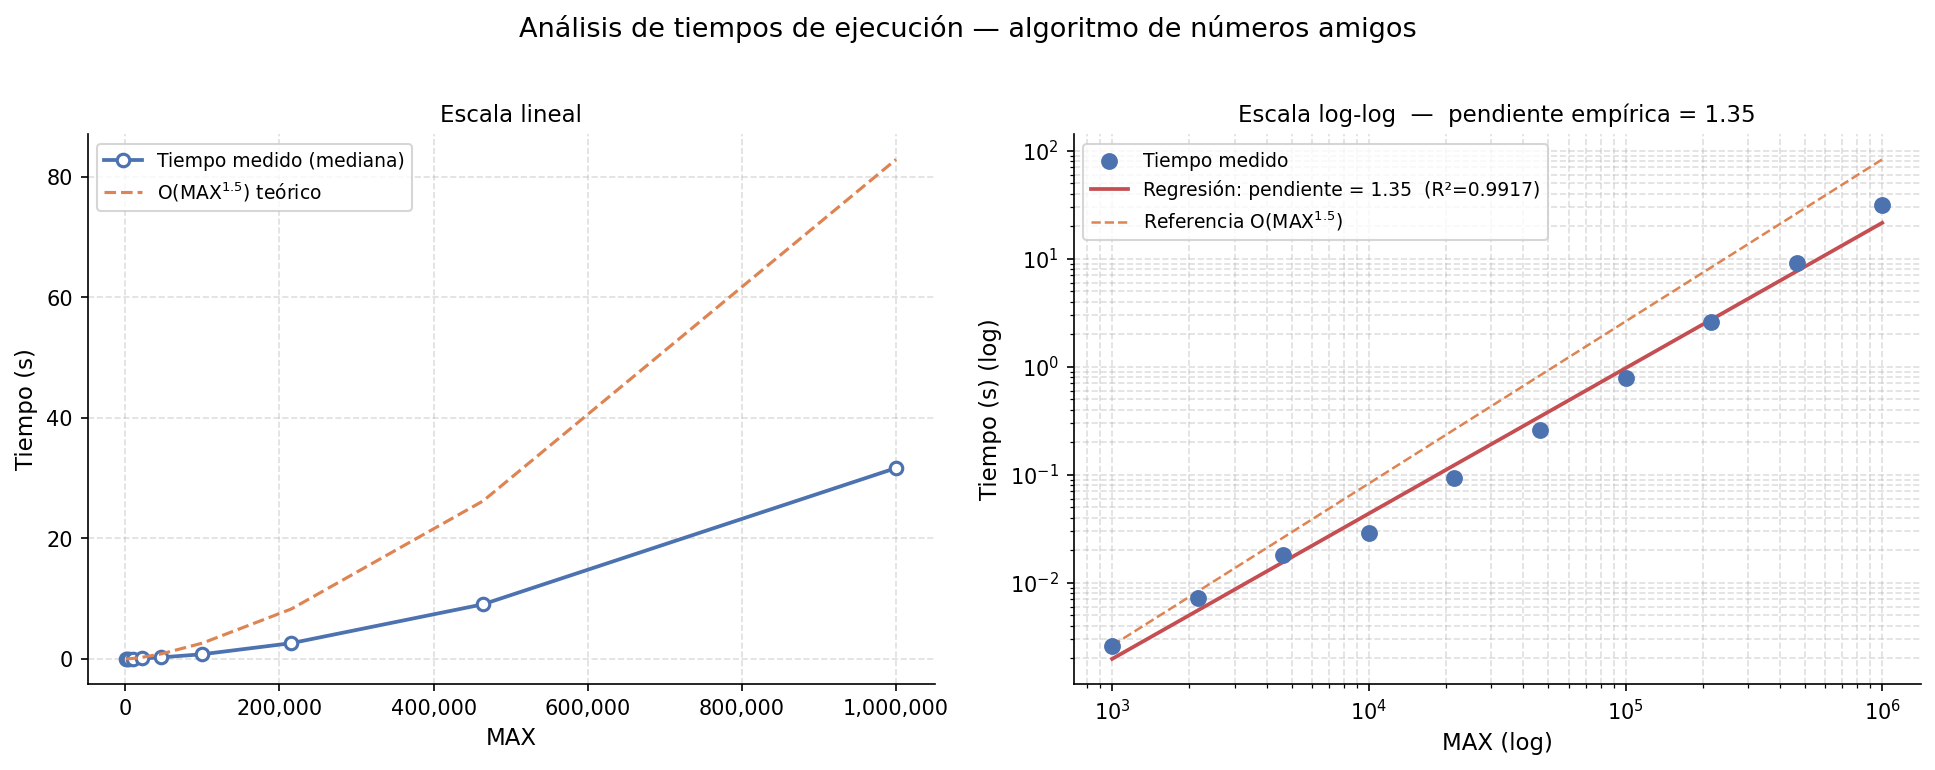
\includegraphics[width=0.9\textwidth]{../graficos/tiempos_ejecucion.png}
    \caption{Análisis de tiempos de ejecución del algoritmo de búsqueda de
             divisores. Panel izquierdo: escala lineal con curva teórica
             $\mathcal{O}(\text{MAX}^{1.5})$. Panel derecho: escala log-log
             con regresión lineal (pendiente~$= 1.35$, $R^{2} = 0.9917$).}
    \label{fig:tiempos_busqueda_divisores}
\end{figure}

\subsubsection{Comparación: Criba vs Búsqueda de Divisores}

Cuando se utiliza una versión optimizada utilizando el método de la criba para calcular sumas de divisores de manera eficiente, esta aproximación demostró una mejora significativa en el rendimiento para limites aun mayores.
Estas son las mediciones comparativas de estas ultimas dos mejoras al algoritmo:

\begin{table}[h]
\centering
\begin{tabular}{|c|c|c|c|}
\hline
\textbf{n} & \textbf{Criba (s)} & \textbf{Búsqueda Divisores (s)} & \textbf{Ratio BD/Criba} \\
\hline
1,000 & 0.0012 & 0.0019 & 1.6 \\
2,500 & 0.0040 & 0.0059 & 1.5 \\
5,000 & 0.0072 & 0.0109 & 1.5 \\
7,500 & 0.0086 & 0.0191 & 2.2 \\
10,000 & 0.0117 & 0.0287 & 2.4 \\
150,000 & 0.3803 & 1.4948 & 3.9 \\
200,000 & 0.4987 & 2.2894 & 4.6 \\
250,000 & 0.6784 & 3.3090 & 4.9 \\
\hline
\end{tabular}
\caption{Comparación de rendimiento entre algoritmos}
\label{tab:comparacion}
\end{table}

\subsection{Análisis de Complejidad}
El análisis experimental reveló diferencias en la complejidad algorítmica dependiendo del algoritmo utilizado:

\begin{itemize}
    \item \textbf{Algoritmo de Búsqueda de Divisores}: Complejidad $O(n*sqrt(n))$
    \item \textbf{Algoritmo de Criba}: Complejidad $O(n*log(n))$
\end{itemize}

La reducción en el exponente de complejidad del método de criba explica la mejora progresiva observada en el rendimiento, que alcanza hasta 4.9 veces mejor para $n = 250,000$.

\subsection{Visualización de Resultados}

Se generaron múltiples gráficos para ilustrar el comportamiento de los algoritmos:

\subsubsection{Comparación de Rendimiento Directo}
\begin{figure}[h]
    \centering
    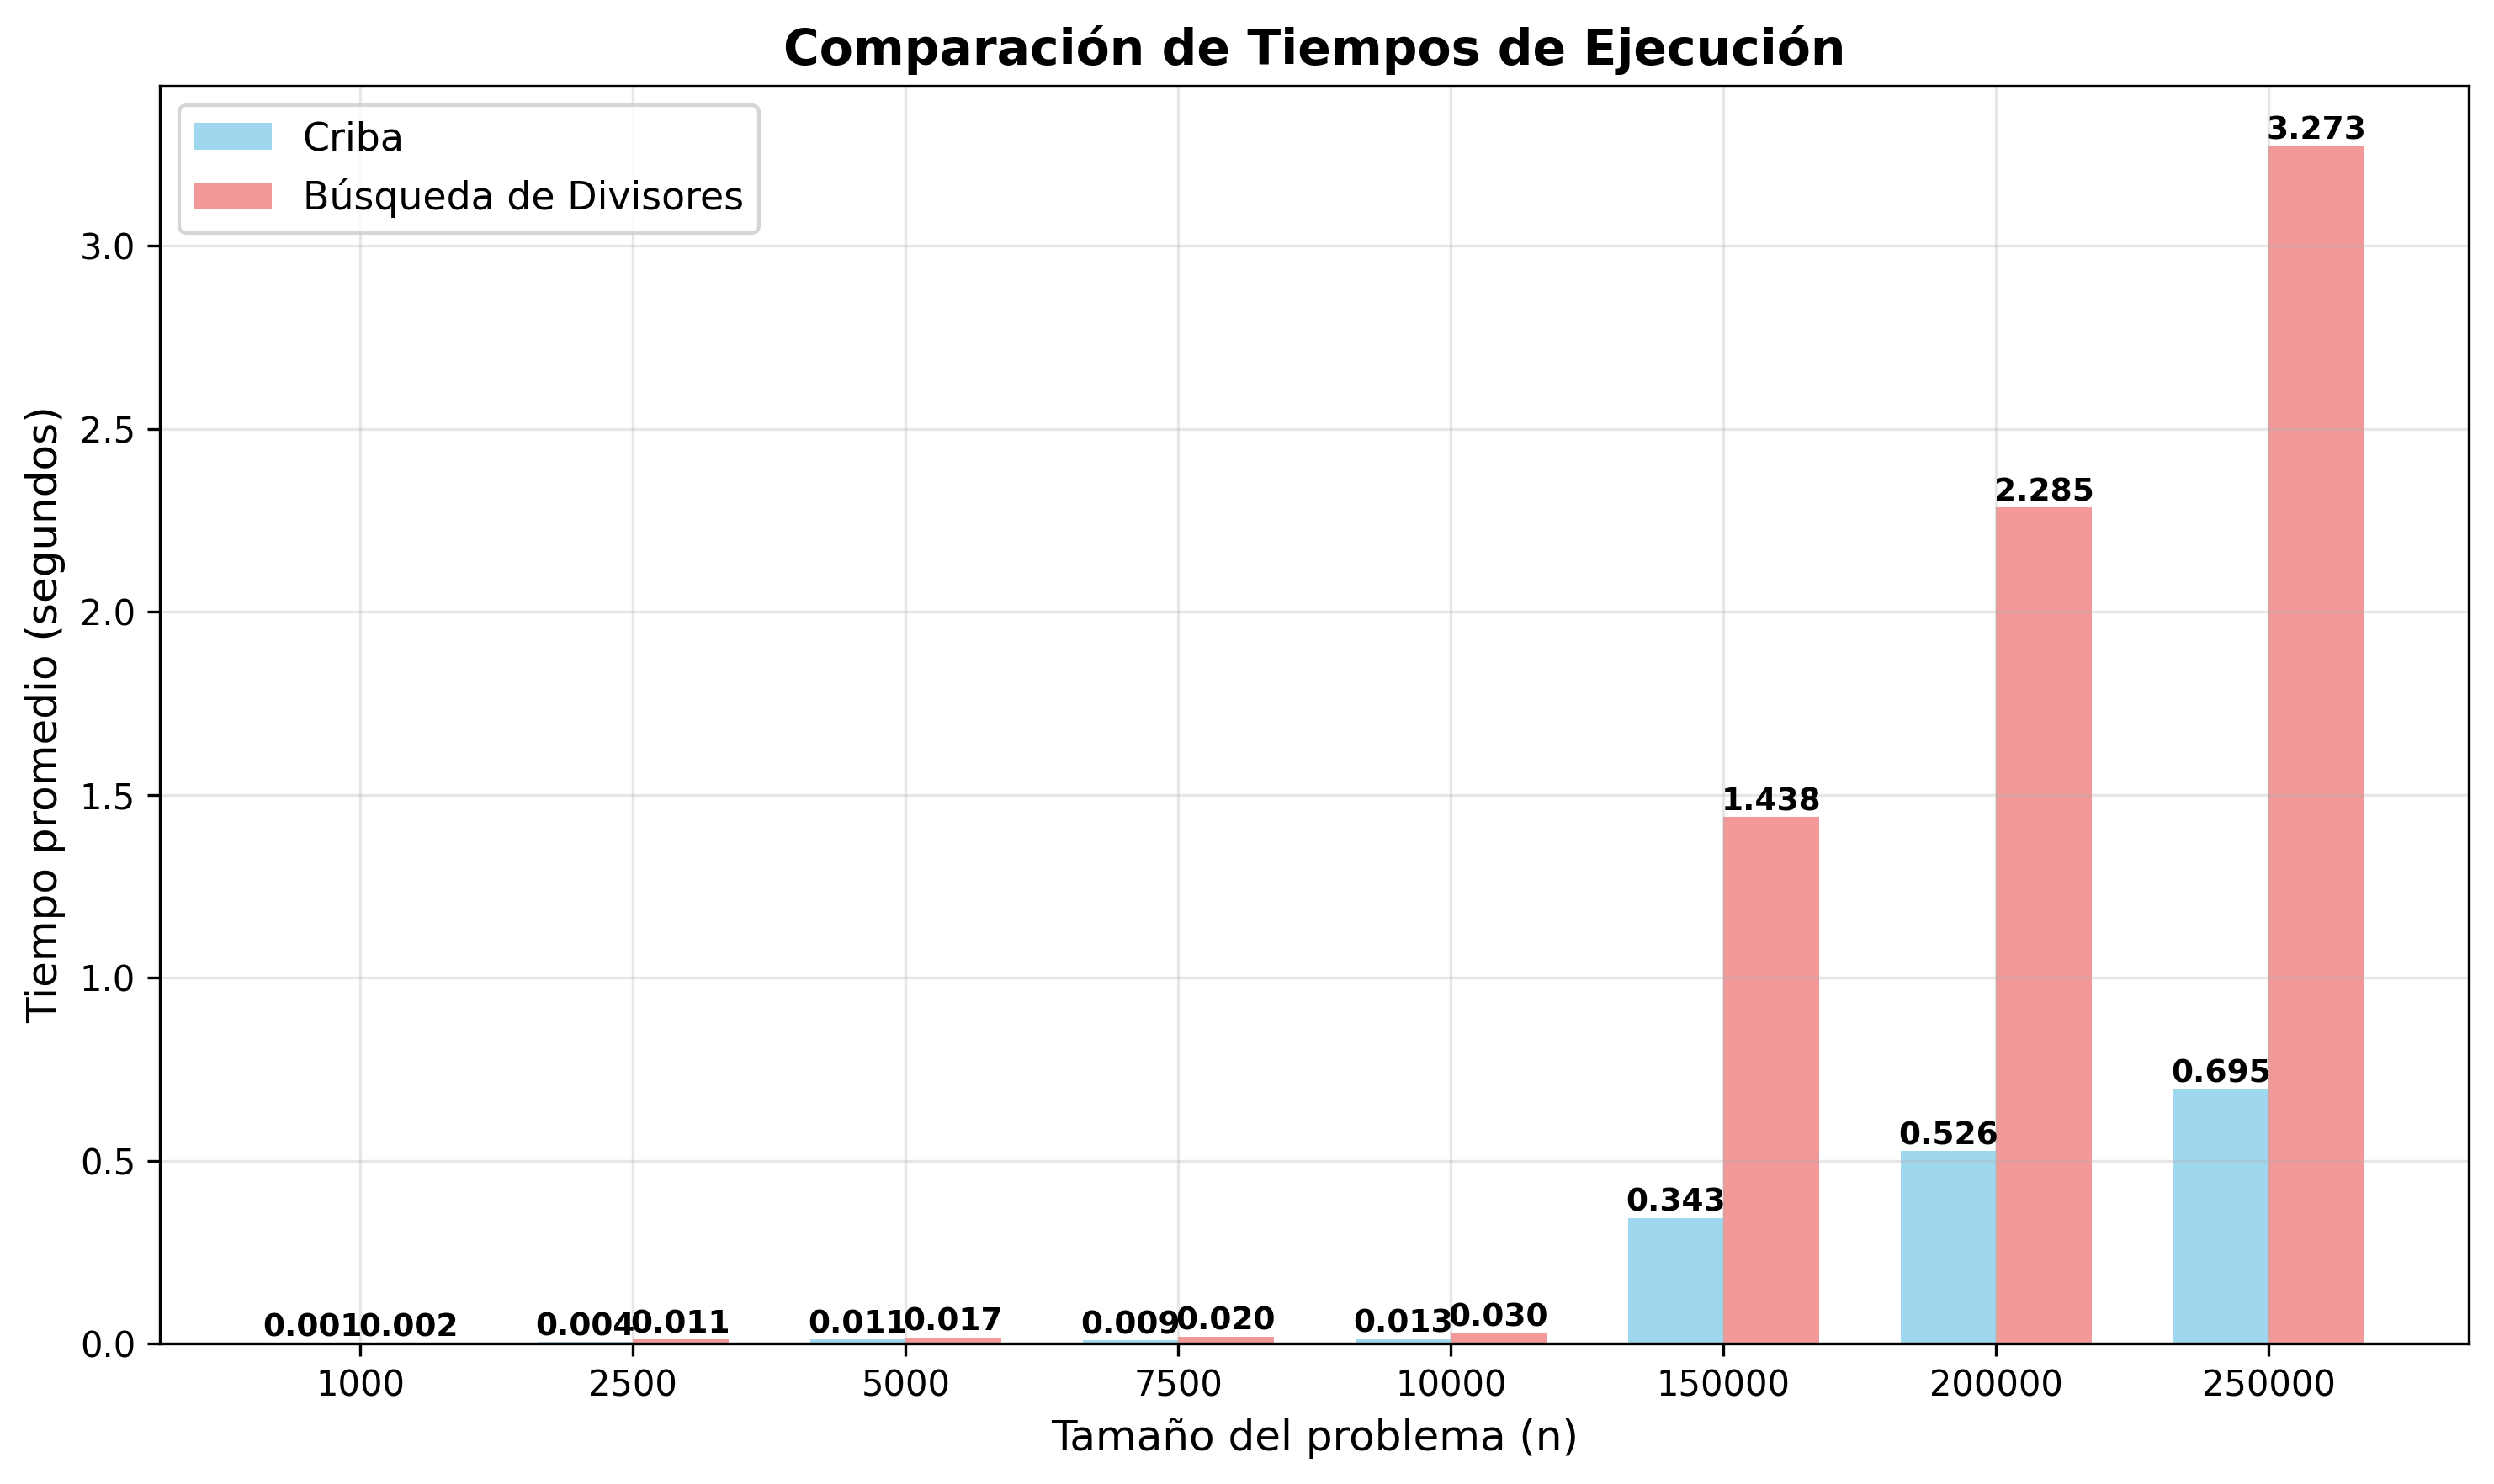
\includegraphics[width=0.8\textwidth]{../graficos/01_comparacion_barras.png}
    \caption{Comparación de tiempos de ejecución entre algoritmos de criba y búsqueda de divisores}
    \label{fig:comparacion_barras}
\end{figure}

Este gráfico busca mostrar de manera visual la diferencia directa en los tiempos de ejecución entre ambos algoritmos para diferentes valores de $n$, permitiendo apreciar claramente la superioridad del método de criba.

\subsubsection{Evolución Temporal del Rendimiento}
\begin{figure}[h]
    \centering
    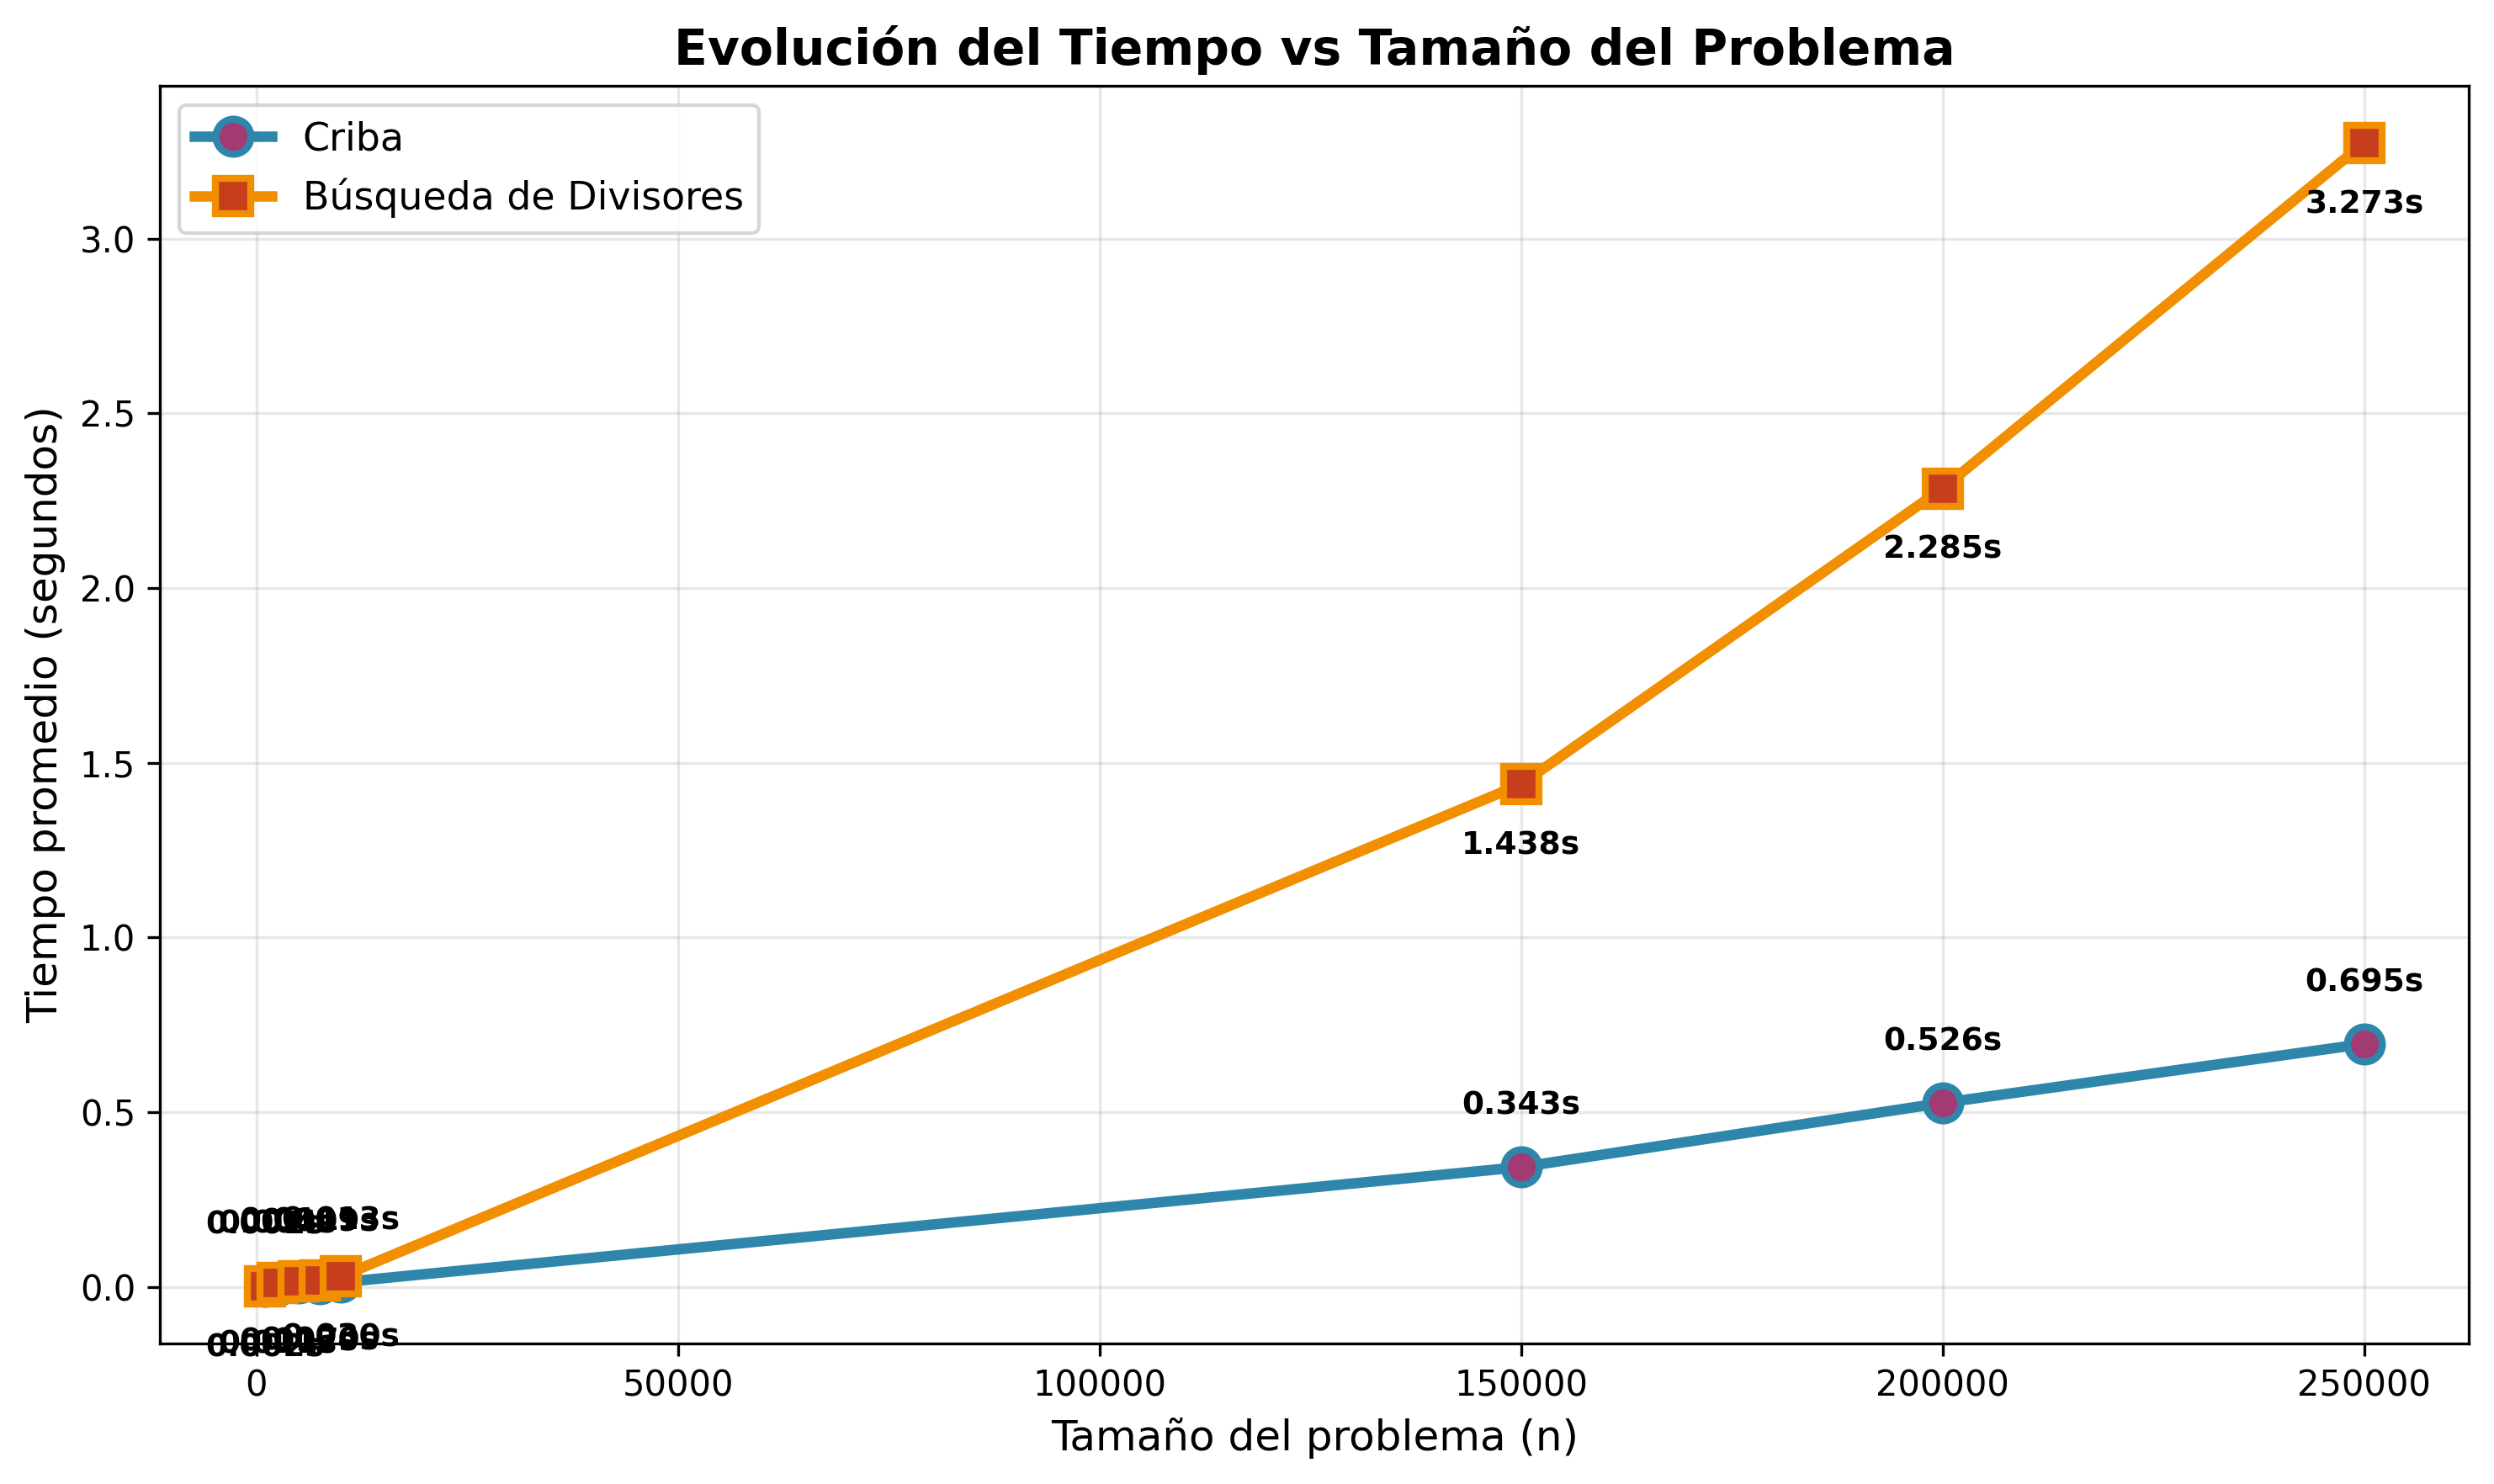
\includegraphics[width=0.8\textwidth]{../graficos/02_evolucion_lineas.png}
    \caption{Evolución temporal del rendimiento según el tamaño del problema}
    \label{fig:evolucion_lineas}
\end{figure}

Esta visualización busca ilustrar cómo evolucionan los tiempos de ejecución a medida que aumenta el tamaño del problema, mostrando las diferentes tasas de crecimiento entre ambos algoritmos y destacando la escalabilidad del método de criba.

\subsubsection{Análisis de Complejidad Algorítmica}
\begin{figure}[h]
    \centering
    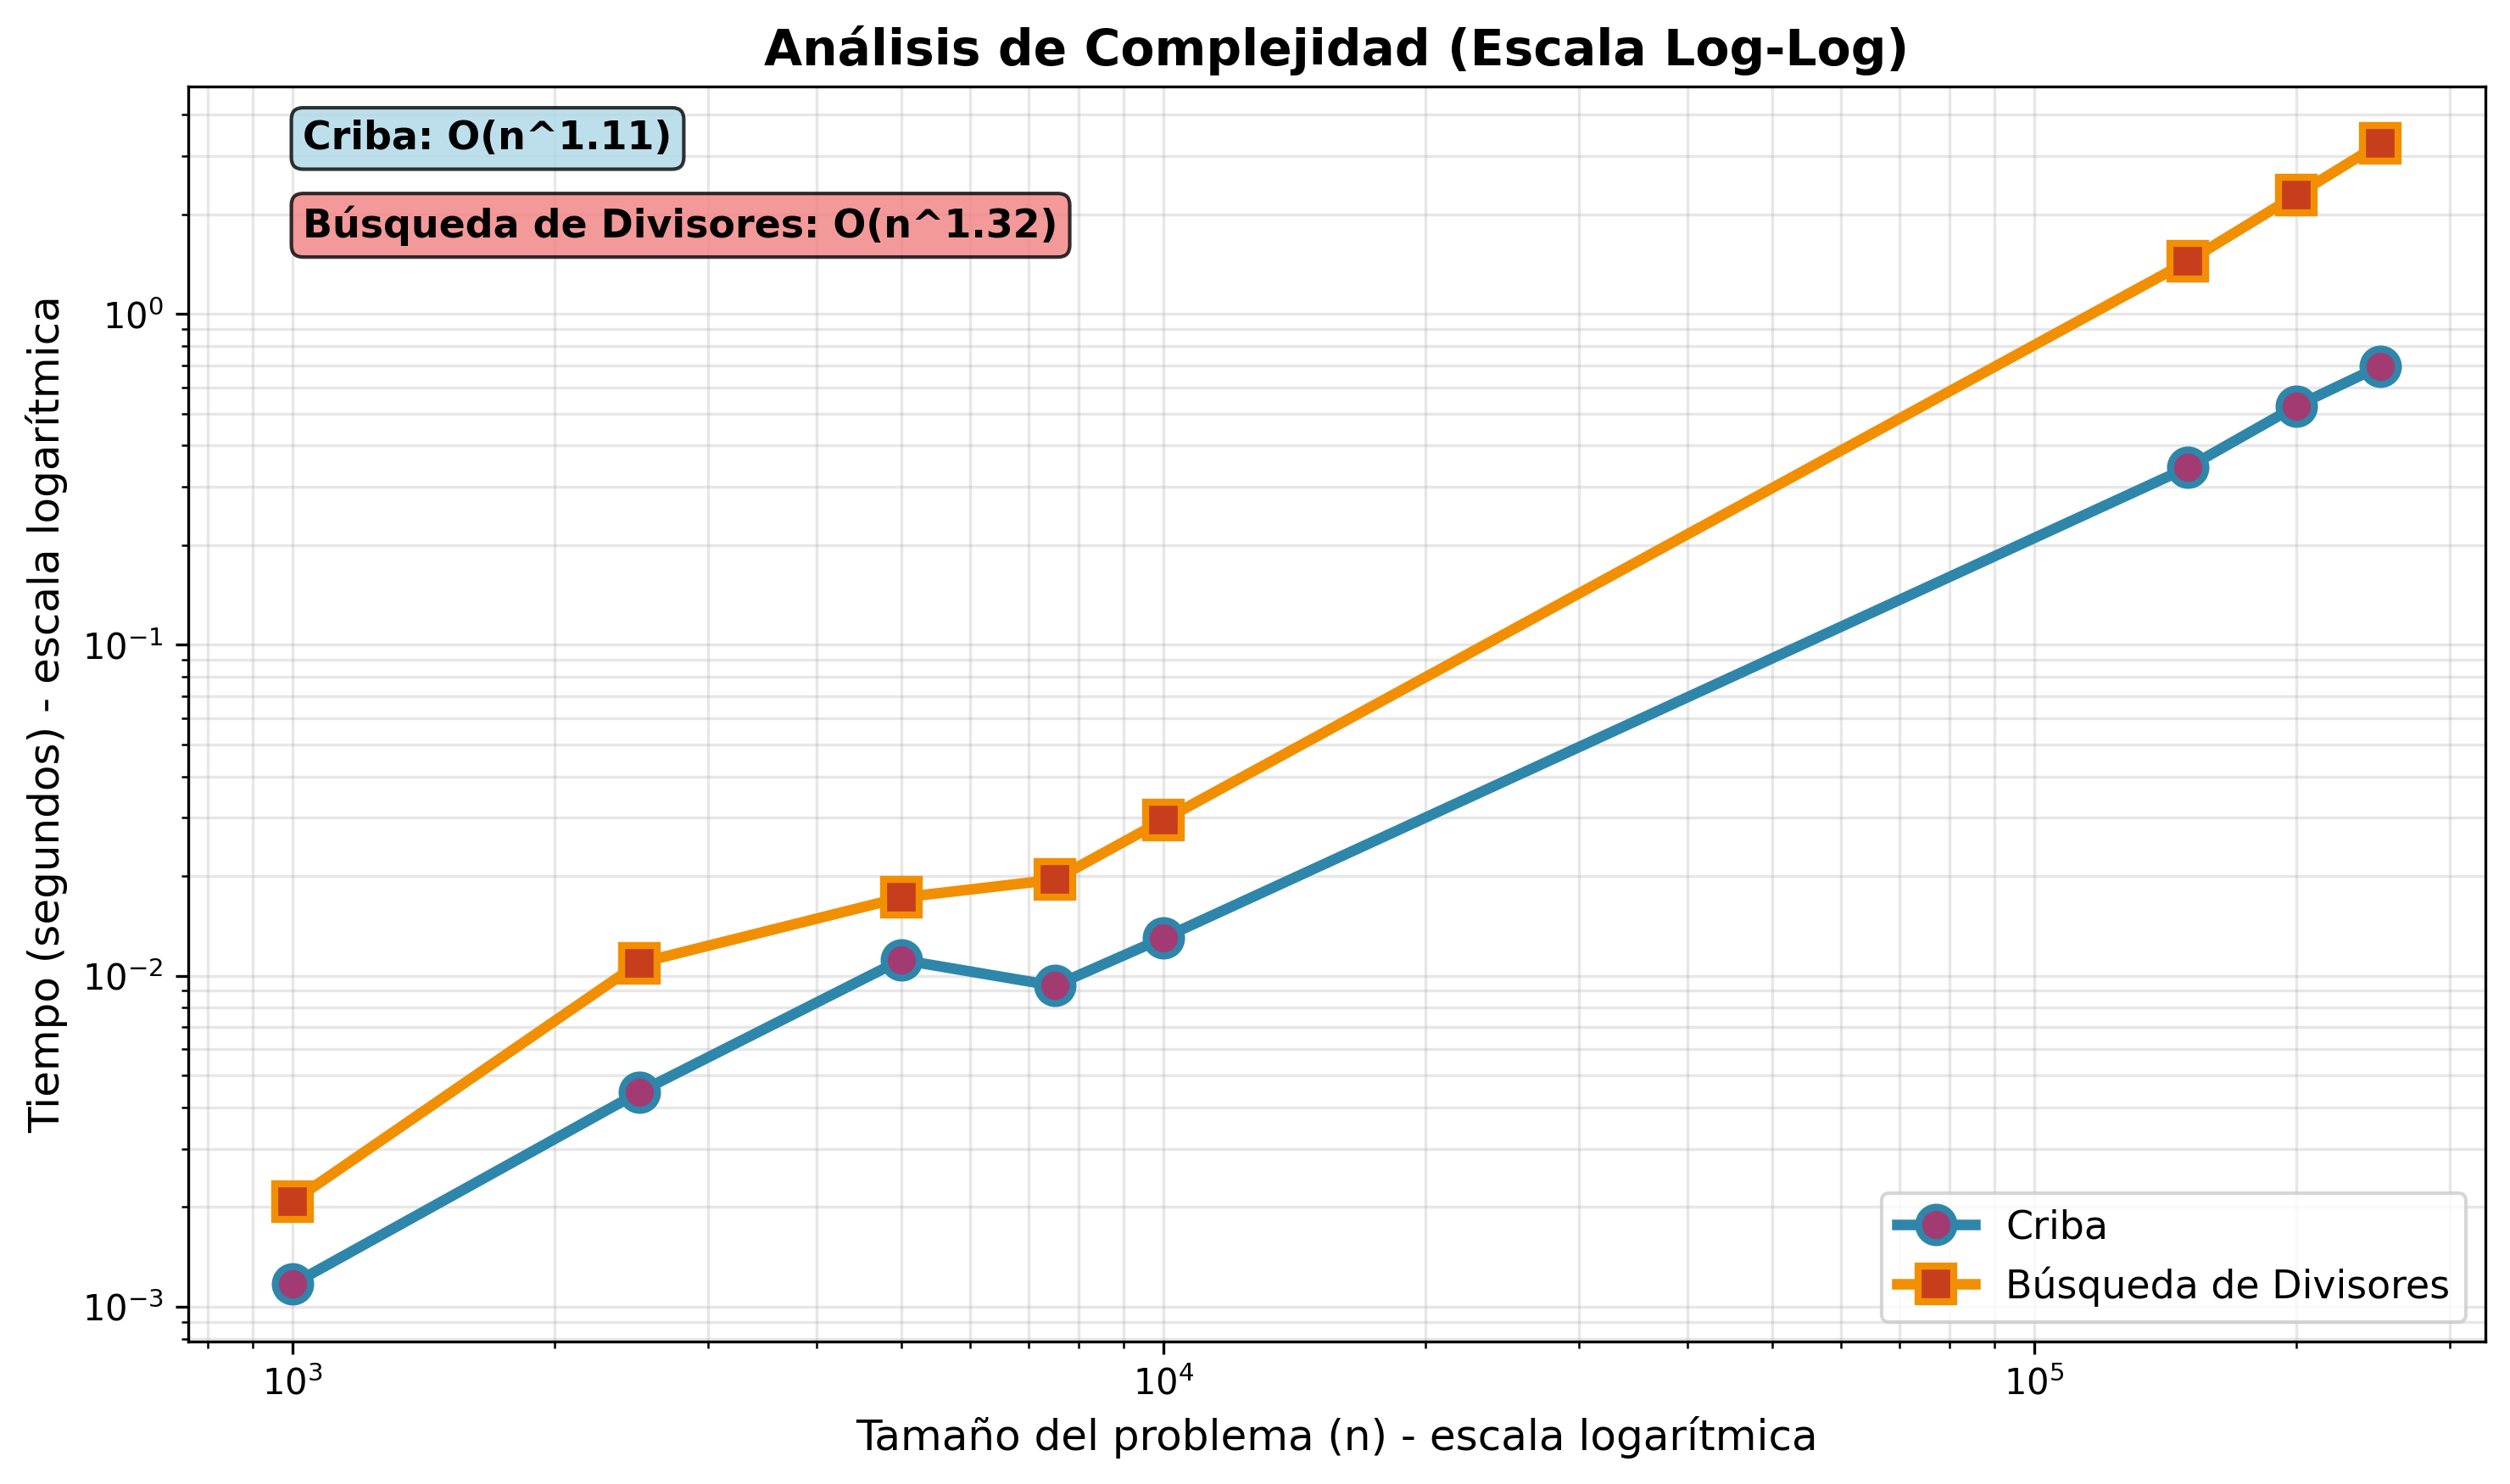
\includegraphics[width=0.8\textwidth]{../graficos/03_analisis_complejidad.png}
    \caption{Análisis de complejidad algorítmica en escala logarítmica}
    \label{fig:analisis_complejidad}
\end{figure}

Este gráfico busca demostrar experimentalmente las complejidades teóricas de ambos algoritmos mediante el análisis en escala log-log, donde las pendientes confirman las complejidades $O(n*sqrt(n))$ para búsqueda de divisores y $O(n*log(n))$ para criba.

\subsubsection{Análisis Avanzado de Eficiencia}
\begin{figure}[h]
    \centering
    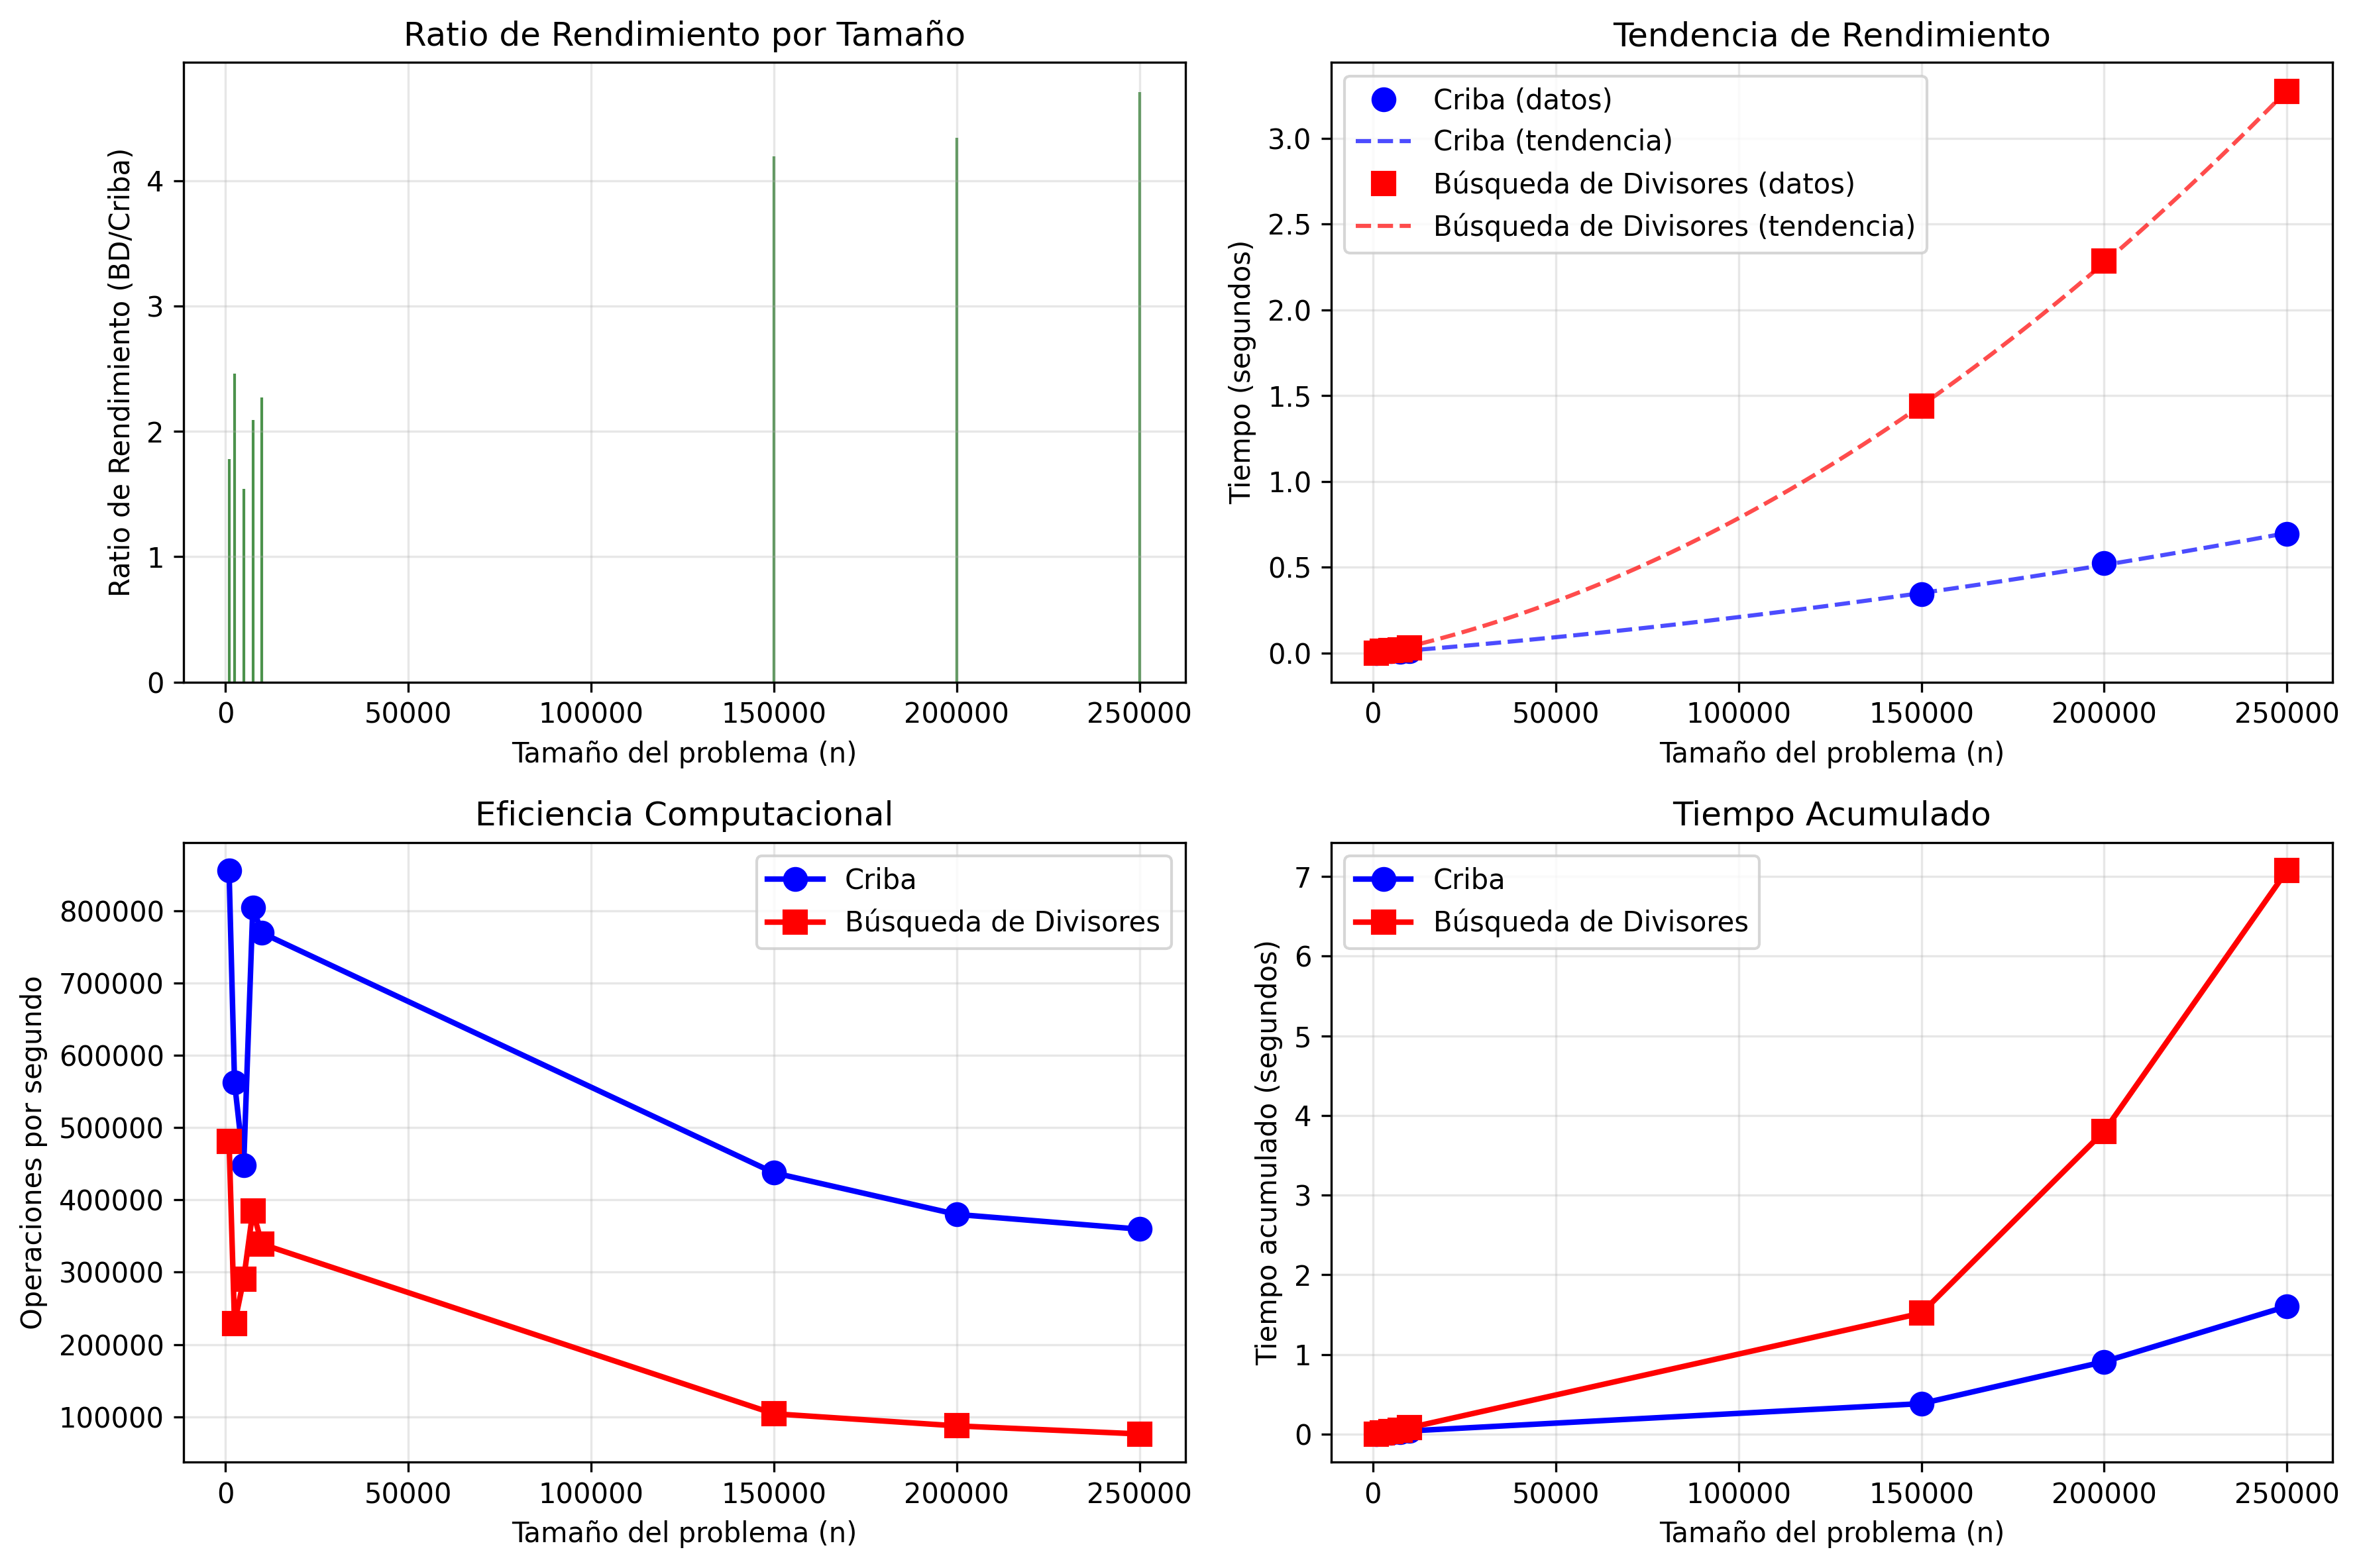
\includegraphics[width=0.9\textwidth]{../graficos/04_analisis_avanzado.png}
    \caption{Análisis avanzado de rendimiento: eficiencia y tendencias}
    \label{fig:analisis_avanzado}
\end{figure}

Esta visualización busca proporcionar un análisis comprehensivo de métricas adicionales de eficiencia, incluyendo tasas de operaciones por segundo y tendencias de mejora relativa, complementando el análisis básico de tiempos de ejecución.
